\documentclass[hyperref={pdfpagelabels=false},table]{beamer}
\usepackage{../estilo-apresentacao/slides-utfpr}

%\hypersetup{pdfpagemode=FullScreen}   %%% para deixar no modo de tela cheia
\beamertemplatenavigationsymbolsempty   %%% para não mostrar ícones de navegação no canto direito inferior

% Nome da disciplina - informação que somente aparece nas propriedades do arquivo PDF
\subject{Desenvolvimento de Aplicaç\~{o}es Distribu\'{i}das - UTFPR}

\title[Desenv. Apl. Distribu\'{i}das - AD23S - 2018/2]{Desenvolvimento de Aplicaç\~{o}es Distribu\'{i}das}
\subtitle{Aula 7: Estudo de Caso: Sockets TCP em Java
}
\author[Prof. Dr. F\'{a}bio Favarim]{Prof. Dr. F\'{a}bio Favarim \texorpdfstring{\\ \footnotesize{favarim@utfpr.edu.br}}{}}
\institute[UTFPR]{ 
\small{\textbf{Universidade Tecnológica Federal do Paraná}}\\
C\^{a}mpus Pato Branco
}

\date{27 de Agosto de 2018}

\begin{document}

\frame{\titlepage}

\frame[t]{ \frametitle{Objetivos da Aula}
   \begin{block}{}
      \begin{itemize}
	    \item Estudo de Caso: API Java para Sockets TCP
	    \item Uso de Streams: Array de Bytes, Data e Object
      \end{itemize}
   \end{block}
}

\section{Sockets TCP - Visão Geral}
\frame[t]{ \frametitle{Sockets: TCP - Transfer Control Protocol}
   \begin{figure}
     
\includegraphics[scale=.26]{figs/tcp}
   \end{figure}

   \begin{block}{TCP: Orientado a conexão – Confiável}
      \begin{itemize}
	\item Uma conexão (canal) deve ser estabelecida antes da transmissão dos dados;
	\item Dados são enviados em \textbf{fluxo contínuo (stream)} no \textbf{canal};
	\item Dados não são enviados datagrama a datagrama, mas fragmentados pelo TCP automaticamente em segmentos
	\item A conexão deve ser encerrada após a transmissão dos dados;

	\begin{itemize}
	  \item Basta \textbf{gravar} no stream para enviar uma mensagem
	  \item Basta \textbf{ler} do stream para receber uma mensagem
        \end{itemize}
	\item É \textbf{garantida \alert{a entrega}} dos segmentos
	\item É \textbf{garantida \alert{a ordem} de entrega} dos segmentos
        \end{itemize}
   \end{block}
}


\begin{frame}[fragile]
	\frametitle{Sockets TCP - Funcionamento Geral}
	\textbf{Sockets de Conexão} - O servidor fica aguardando \textbf{conexões} de clientes em um socket em \textbf{porta} específica.

	\begin{figure}
		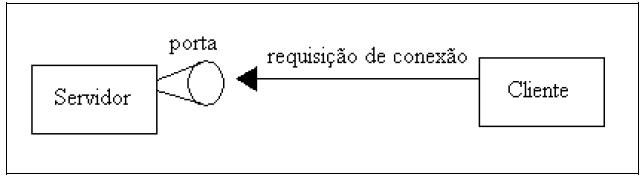
\includegraphics[scale=.26]{figs/tcp-conexao}
	\end{figure}

	\textbf{Socket de comunicação} - Quando aceita a conexão de um cliente, \textbf{outro socket} é criado para a \textbf{comunicação}. 
	\begin{figure}
		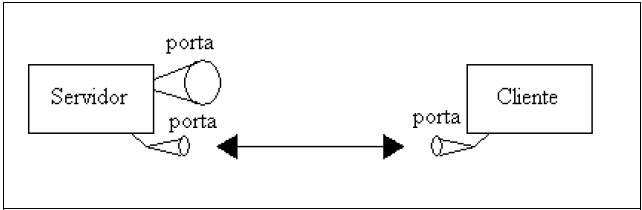
\includegraphics[scale=.26]{figs/tcp-comunicacao}
	\end{figure}

\end{frame}


\begin{frame}[t]\frametitle{Passos de Comunicação com Sockets TCP }
  \begin{block}{Servidor}
    \begin{enumerate}
      \item Criar socket de conexão 
      \item Fica ouviando aguardando conexões de clientes, quando conectar criar socket de comunicação
      \item Cria canais de comunicação (streams) com o cliente (no Java)
      \item Faz a comunicação com o cliente
      \item Fecha socket com o cliente
    \end{enumerate}
  \end{block}

    \begin{block}{Cliente}
      \begin{enumerate}
	\item Cria socket cliente
	\item Cria canais de comunicação (streams) com o servidor (no Java)
	\item Faz a comunicação com o servidor
	\item Fechar socket com o servidor
    \end{enumerate}
  \end{block}
  
\end{frame}


% ------------ Inicio do documento ---------------%
\section{API Java para programação com Sockets TCP}
\subsection{Definições}

\begin{frame}[t]\frametitle{API Java para programação com Sockets}
  \begin{block}{Pacote \textbf{java.net}, principais classes:}
    \begin{itemize}
      \item \textbf{UDP:} DatagramPacket e DatagramSocket;
      \item \textbf{TCP:} Socket e ServerSocket;
      \item Outras: obtenção endereço IP e porta de um pacote, entre outras coisas.
     \end{itemize}
  \end{block}
\end{frame}



\subsection{Comandos Básicos}
\begin{frame}[fragile]
	\frametitle{Sockets TCP (Java) - Comandos Básicos}

	Criação de Socket de Conexão (Para aguardar por conexões)
	\begin{lstlisting}
    	ServerSocket conexao = new ServerSocket(porta, [tamanho_fila]);
		// tamanho_fila = maximo de pedidos de conexoes que e mantido para o socket
	\end{lstlisting} 
	
	
	Criação do Socket de Comunicação / Estabelecer canal comunicação
	\begin{lstlisting}
	// Lado Servidor
  	Socket socket = conexao.accept();

	// Lado Cliente
	Socket socket = new Socket(host, porta);

	\end{lstlisting} 

	Fechar Socket de Comunicação
	\begin{lstlisting}
		socket.close();  // conexao.close();
	\end{lstlisting} 

\end{frame}

\begin{frame}[fragile]
	\frametitle{Sockets TCP (Java) - Comandos Básicos}

	Criar fluxos (streams) de entrada e saída de dados, conforme o tipo de dados.

	\begin{itemize}
		\item Streams são canais de comunicação entre um programa e uma fonte de dados
		\item As fontes de dados podem ser: arquivos, trechos de memória e conexões de rede
		\item Em Java não importa qual é a fonte, a forma de usar é a mesma
		\item Em Java há vários classes para manipulação de \textbf{streams}, vamos usar três:
		\begin{itemize}
			\item Tipos básicos (int, String, double...)
			\item Objetos
			\item Array de Bytes
		\end{itemize}
	\end{itemize}
\end{frame}


\begin{frame}[fragile]
	\frametitle{Sockets TCP (Java) - Comandos Básicos}

	Criar streams com tipos básicos (DataInputStream/DataOutputStream)
	\begin{lstlisting}
		DataInputStream in = new DataIntputStream(socket.getInputStream());
		DataOutputStream out = new DataOutputStream(sockeet.getOutputStream());
	\end{lstlisting} 

	Enviar dados para o stream
	\begin{lstlisting}
		out.writeUTF("Alo pessoal");
		out.writeDouble(15.5);
		out.writeInt(15);
	\end{lstlisting} 

	Receber dados do stream
	\begin{lstlisting}
		String resposta = in.readUTF();
		double resposta = in.readDouble();
		int resposta = in.readInt();
	\end{lstlisting} 
\end{frame}

\begin{frame}[fragile]
	\frametitle{Sockets TCP (Java) - Comandos Básicos}

	Criar streams de Objetos (ObjectInputStream/ObjectOutputStream)
	\begin{itemize}
		\item Um objeto só pode ser gravado/lido se implementar a interface Serializable
		\item Um objeto serializável é aquele cuja representação pode ser transformado em bytes e poderá ser armazenado em disco ou transmitido via stream. 
	\end{itemize}

	\begin{lstlisting}
		ObjectInputStream in = new ObjectIntputStream(socket.getInputStream());
		ObjectOutputStream out = new ObjectOutputStream(socket.getOutputStream());
	\end{lstlisting} 

	Enviar dados para o stream
	\begin{lstlisting}
		out.writeObject(objeto);
	\end{lstlisting} 

	Receber dados do stream
	\begin{itemize}
		\item Deve-se fazer o cast para o tipo de objeto específico
	\end{itemize} 
	\begin{lstlisting}
		TipoObjeto resposta = (TipoObjeto) in.readObject();
	\end{lstlisting} 
\end{frame}

\subsection{Programas}

\subsection{Servidor}
\begin{frame}[fragile]
	\frametitle{Sockets TCP (Java) - Programa Servidor}

	\begin{lstlisting}
		//Passo 1: aguarda conexao
		ServerSocket conexao = new ServerSocket(porta, tamanho_fila);
		do{
		  //Passo 2: aguarda conexao do cliente
		  Socket socket = conexao.accept();

		  //Passo 3: obtem o stream de entrada e saida
		  DataInputStream in = new DataInputStream(socket.getInputStream());
		  DataOutputStream out = new DataOutputStream(socket.getOutputStream());
		
		  //Passo 4: realiza a comunicacao conforme o protocolo
		  String data = in.readUTF();
		  out.writeUTF(data);

		  //Passo 5: fecha o socket com o cliente
		  socket.close();
		} while(notExit());

		//Passo 6: fecha o socket servidor
		serverSocket.close();
	\end{lstlisting} 
\end{frame}

\subsection{Cliente}
\begin{frame}[fragile]
	\frametitle{Sockets TCP (Java) - Programa Cliente}

	\begin{lstlisting}
		InetAddress address = InetAddress.getbyName(name);

		//Passo 1: Conecta o socket a porta do servidor
		Socket socket = new Socket(address,port);
            
		//Passo 2: cria streams entrada e saida
		DataOutputStream out = new DataOutputStream(socket.getOutputStream());
		DataInputStream in = new DataInputStream(socket.getInputStream());

		//Passo 3: realiza a comunicacao conforme protocolo
		out.writeUTF(request);
		String resposta = in.readUTF();

		//Passo 4: fecha o socket
		socket.close();
	\end{lstlisting} 
\end{frame}


\begin{frame}[fragile]
	\frametitle{Código Exemplo}
	\begin{itemize}   
	 \item Pegar no moodle os códigos de exemplo
	 \item A aplicação exemplo trata-se de uma aplicação onde o cliente envia uma mensagem para o servidor e o servidor devolve (faz eco) a mesma mensagem ao  cliente.
	\end{itemize}
\end{frame}


\section{Exercícios}
\frame[t]{ \frametitle{Exercícios}
	 \begin{itemize}
		\item Lista de Exercícios Sockets TCP
	 \end{itemize}
}

\frame[t]{ \frametitle{Próxima aula}
	 \begin{itemize}
	  \item Threads em Sistemas Distribuídos
	 \end{itemize}
}

\end{document}
